\documentclass[tikz,border=2pt]{standalone}
\usepackage{amsmath}
\usepackage{pgfplots}
\pgfplotsset{compat=1.18}
\usetikzlibrary{arrows.meta}
\begin{document}
% A data frame is a set of equal-length column vectors, each with its own type; a row is one
% observation. df has Name (chr), Height and Weight (num) and the added column ID (num).
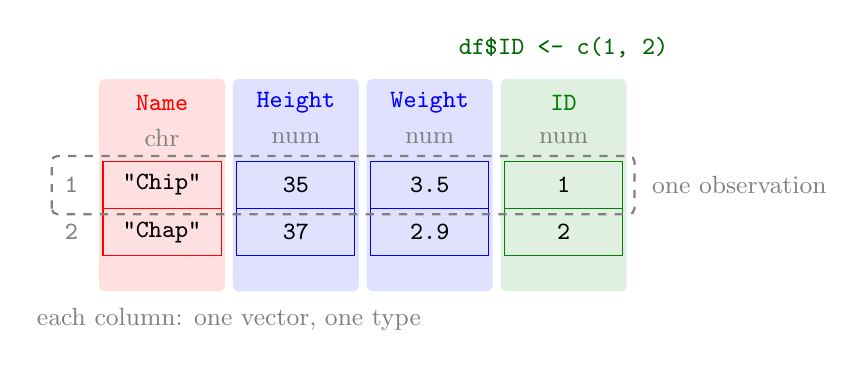
\begin{tikzpicture}[font=\small, >={Latex[length=2mm]},
  cell/.style={draw, minimum width=15mm, minimum height=6mm, inner sep=0pt, font=\small\ttfamily, text=black}]
  \foreach \name/\type/\a/\b/\col [count=\i] in {
      Name/chr/"Chip"/"Chap"/red,
      Height/num/35/37/blue,
      Weight/num/3.5/2.9/blue,
      ID/num/1/2/green!50!black} {
    \pgfmathsetmacro{\x}{1.7*\i}
    \fill[\col!12, rounded corners=2pt] (\x-0.8,-0.45) rectangle (\x+0.8,2.25);
    \node[font=\small\ttfamily\bfseries, text=\col] at (\x,1.95) {\name};
    \node[gray] at (\x,1.5) {\type};
    \node[cell, draw=\col] at (\x,0.9) {\a};
    \node[cell, draw=\col] at (\x,0.3) {\b};
  }
  \node[gray, font=\small\ttfamily] at (0.55,0.9) {1};
  \node[gray, font=\small\ttfamily] at (0.55,0.3) {2};
  \draw[gray, dashed, thick, rounded corners=2pt] (0.3,0.53) rectangle (7.7,1.27);
  \node[gray, anchor=west] at (7.8,0.9) {one observation};
  \node[gray] at (2.55,-0.8) {each column: one vector, one type};
  \node[green!40!black, font=\small\ttfamily] at (6.8,2.65) {df\$ID <- c(1, 2)};
\end{tikzpicture}
\end{document}
